\chapter{Implementácia}

\section{Vývoj s pomocou príkazového riadku}

Ruby on Rails má zabudovanú konzolovú aplikáciu, ktorá uľahčuje vývoj pomocou príkazov. Ak zadáme \emph{\$ rails help} tak dostaneme nasledovný výstup

\begin{minted}{bash}
$ rails help
Usage: rails COMMAND [ARGS]

The most common rails commands are:
 generate    Generate new code (short-cut alias: "g")
 console     Start the Rails console (short-cut alias: "c")
 server      Start the Rails server (short-cut alias: "s")
 test        Run tests (short-cut alias: "t")
 dbconsole   Start a console for the database specified in config/database.yml
             (short-cut alias: "db")
 new         Create a new Rails application. "rails new my_app" creates a
             new application called MyApp in "./my_app"

 ...
\end{minted}

\clearpage
Tieto príkazy dokážu urýchliť vývoj, keďže nemusíme konfigurovať štruktúru adresárov, sťahovať repozitáre Ruby on Rails a vytvárať súbory ručne alebo poskytuje iné nástroje.
Najdôležitejšie pri vývoji sú príkazy \emph{rails server}, \emph{rails console} a \emph{rails new}. 


\textbf{\emph{\$ rails server}} -- ako meno napovedá spustí server, ktorý je určený v súbore balíčkov -- \emph{Gemfile}, pričom môžeme flagmi špecifikovať na akom porte a adrese sa má aplikácia spustiť.

\textbf{\emph{\$ rails console}} -- spúšťa interaktívnu konzolu, kde vývojár môže otestovať správanie jednotlivých komponentov webovej apliácie, bez toho aby musel spúšťať server a testovať cez užívateľské rozhranie v prehliadači.

\textbf{\emph{\$ rails new my\_app}} -- sa nepoužíva príliš často, keďže tento príkaz vytvára novú aplikáciu aj s celou jej štruktúrou. Zároveň nastaví a stiahne všetky závislosti. Pri vytváraní sa môžu určité závislosti, ako použitá databáza alebo použitý JavaScript-ový framework pomocou flagov (napríklad \emph{-d=postgresql} ak chceme použiť pri všetkých štádiach vývoja databázu PostgreSQL.

Ďalšia časť príkazov sú generátory súborov ako bolo spomenuté v kapitole 2.2. Generátory vytvárajú iba kostru súboru spolu aj s názvom, kde potom vývojar môže dopísať svoj kód. Všetky typy generátorov súborov môžeme zobraziť pomocou príkazu \emph{\$ rails generate}.

Dôležité príkazy sú pre prácu s migráciami a teda databázou. Keď má vývojár migrácie napísané tak ich potrebuje aby sa podľa nich v databáze vytvorili tabuľky, stĺpce, indexy... Príkazov pre prácu s databázou je mnoho ale pri vývoji som používal najčastejšie nasledujúce:

\begin{minted}{bash}
$ rails db:[COMMAND]
$ rails db:create   # Vytvorí databázu
$ rails db:migrate  # Prevedie všetky migrácie z DSL do databázy
$ rails db:seed     # Vytvorí prichystané objekty do databázy
                    # zo súboru ./db/seeds.rb
$ rails db:rollback # Vráti všetky zmeny z predchádzajúcej migrácie
$ rails db:drop     # Odstráni databázy
\end{minted}

\section{Smerovanie}

Ruby on Rails využíva pri mapovaní URL adries router. Tieto mapovania môže vývojár ľubovoľne meniť a teda priradiť určitú cestu danému controller-u. Všetky tieto cesty sídlia v súbore \emph{./config/routes.rb}. Cesty môžeme priebežne sledovať aj pomocou príkazu \emph{\$ rails routes}. Tu je ukážka definovaných ciest z aplikácie pre podporu rozvrhov:

\begin{minted}{ruby}
Rails.application.routes.draw do
  root "pages#index"
  devise_for :users

  namespace :api do
    post "/teacher/group/course", to: "teacher_group_courses#create"
    delete "/teacher/group/course", to: "teacher_group_courses#destroy"
  end

  resources :courses
  resources :groups
  resources :teachers do
    resources :reports, controller: "teacher_reports" do
      get "/email", to: "teacher_reports#email"
      post "/email", to: "teacher_reports#email_send"
    end
  end
  ...
end
\end{minted}

Existuje niekoľko príkazov ktoré tieto cesty umožňujú vytvárať pomocou a sú nazvané podľa typu HTTP requestu (GET, POST). Keď sú cesty definované pomocou týchto funkcií majú tvar:

\begin{minted}{ruby}
get "/stranka", to: "controller#akcia"
\end{minted}

Kde hash \emph{to: STRING} mapuje cestu na špecifický controller a akciu v ňom. Sú však aj ďalšie špecifické prípady, napríklad domovská stránka aplikácie sa definuje pomocou funkcie \emph{\texttt{root "controller\#akcia"}}

Príkaz \emph{\texttt{resources :symbol}} je v skratkou pre vytváranie REST-ful ciest a cesty vygenerované týmto príkazom vyzerajú nasledujúco:

\begin{minted}{bash}
       NAZOV VERB   CESTA                 CONTROLLER#AKCIA
symbol_index GET    /symbol               symbol#index
             POST   /symbol               symbol#create
  new_symbol GET    /symbol/new           symbol#new
 edit_symbol GET    /symbol/:id/edit      symbol#edit
      symbol GET    /symbol/:id           symbol#show
             PATCH  /symbol/:id           symbol#update
             PUT    /symbol/:id           symbol#update
             DELETE /symbol/:id           symbol#destroy
\end{minted}

V príklade môžeme vidieť aj preddefinovaný príkaz \emph{devise\_for :users}, ktorý je súčasťou balíčka autentifikácie užívateľov nazvaného Devise a vytvára cesty potrebné pre fungovanie tohto balíčka.

Ďalej je použitá aj funkcia \emph{namespace :api ...}, ktorá dokáže zoskupovať podobné príkazy pod spoločnú url, v príklade je to api, čiže všetky cesty budú začínať \emph{\texttt{\/api/cesta}}.

\section{Modely}

\section{Controllery}

\section{Views}


\section{Spracovanie úloh na pozadí}

\section{Generovanie PDF prehľadov}
\section{Odosielanie e-mailov}

\clearpage
\section{Užívateľské rozhranie}

\subsection{Prihlásenie a registrácia}

Pred začatím používania aplikácie sa musí užívateľ najprv prihlásiť alebo registrovať. Všetky podstránky aplikácie sú zabezpečené a užívateľ je presmerovaný pokiaľ nie je prihlásený.

\begin{figure}[!htb]
  \centering
  %\hspace*{-1cm}
  %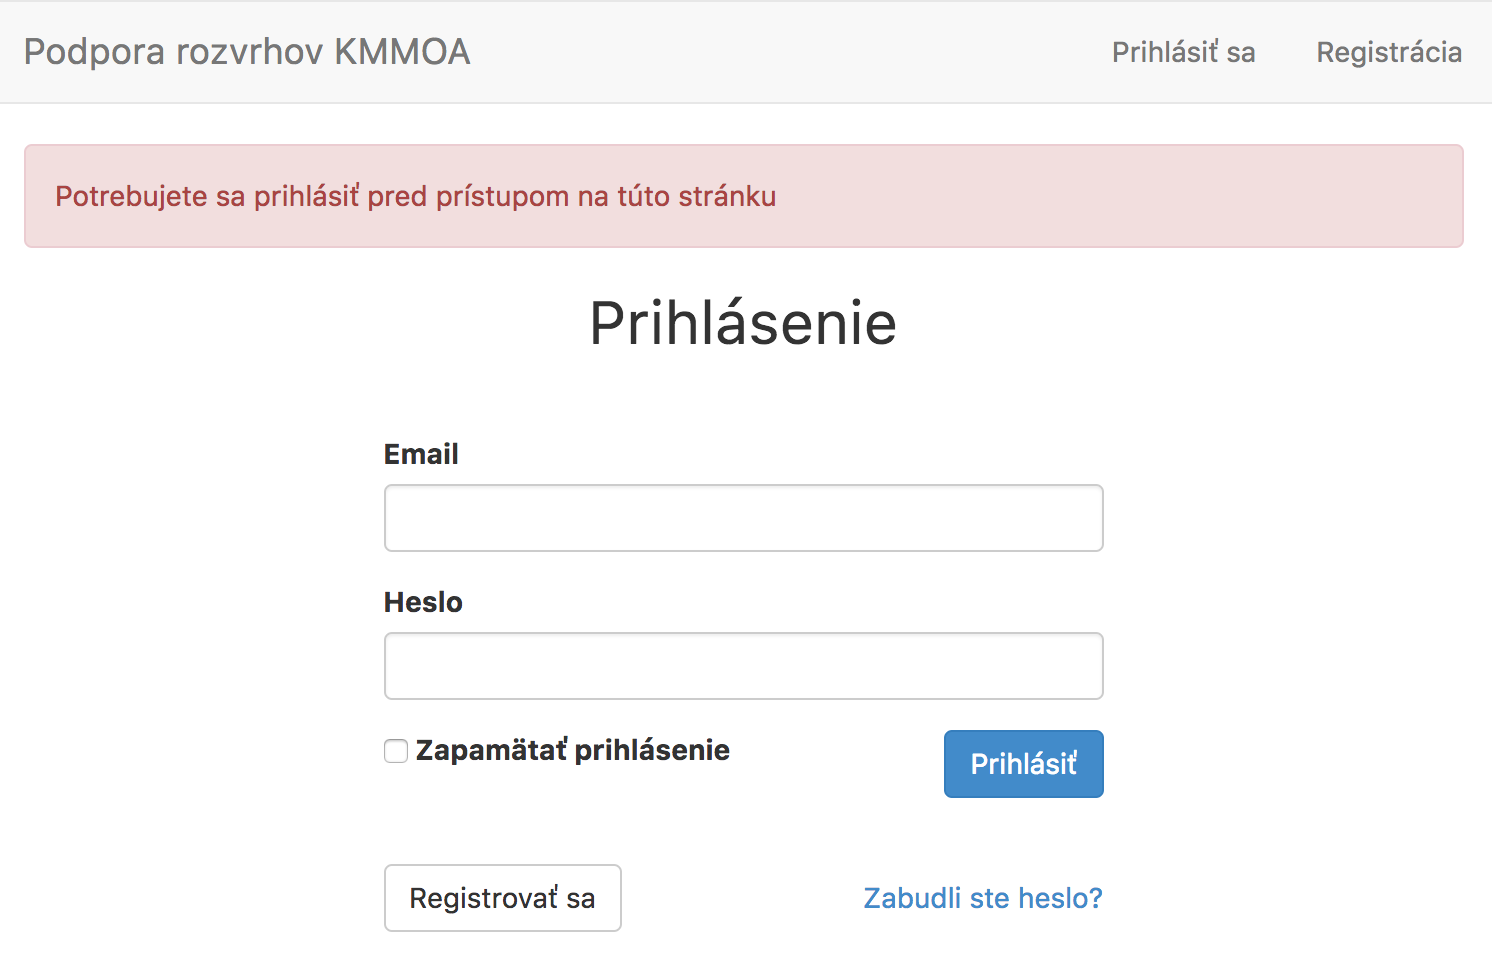
\includegraphics[width=1.1\textwidth]{content/images/login}
  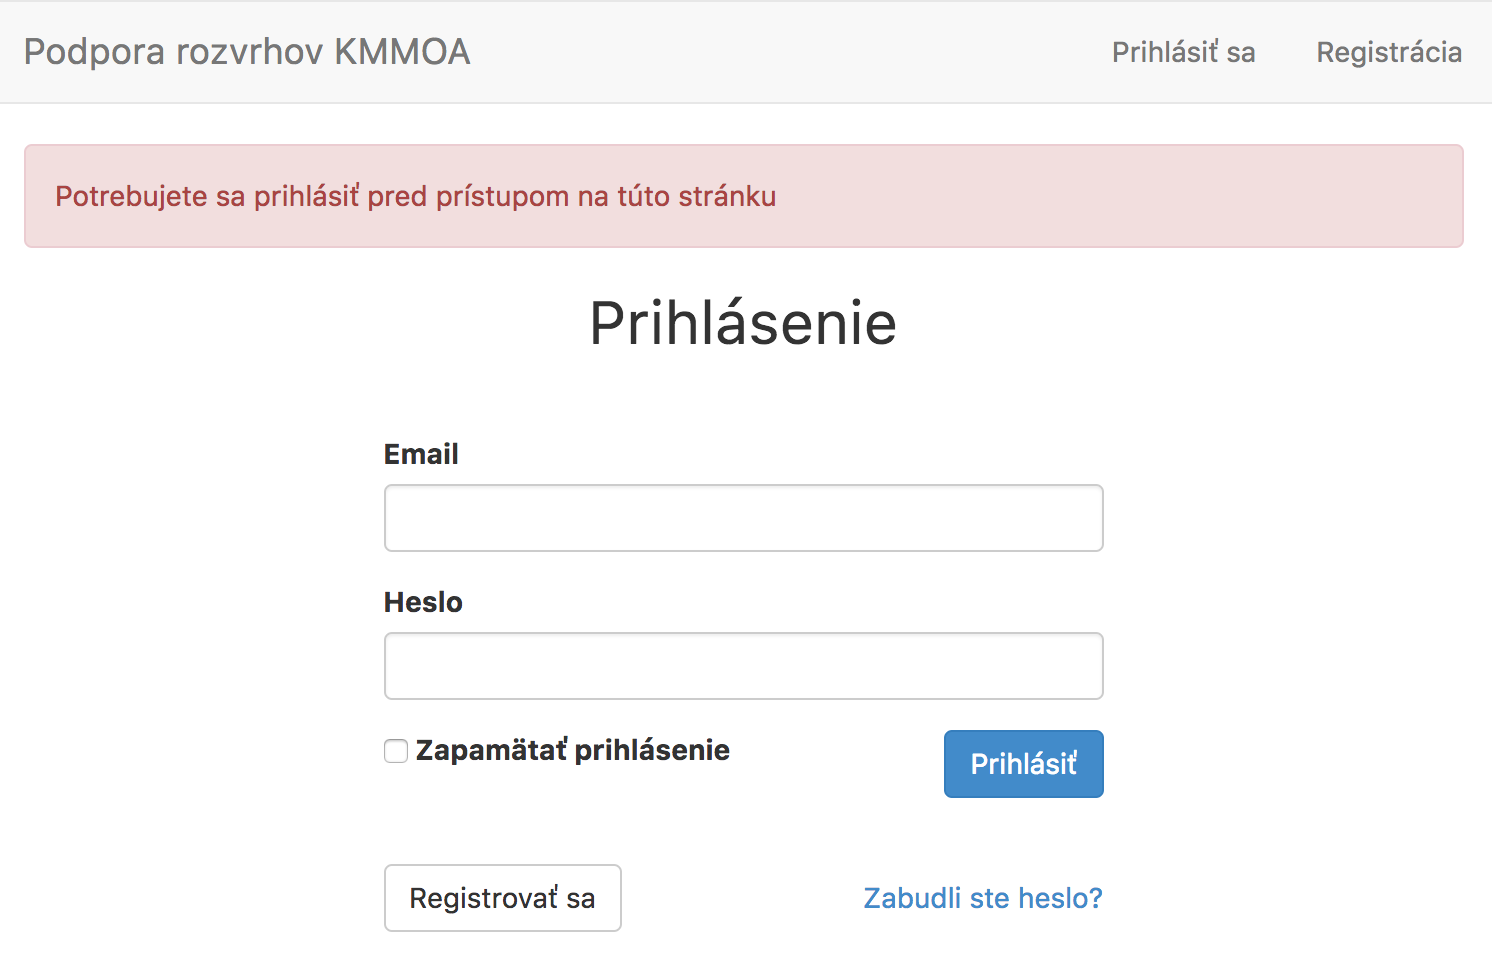
\includegraphics[width=1\textwidth]{content/images/login}
  \caption{Rozhranie pre prihlásenie do aplikácie.}
\end{figure}

Užívatelia si taktiež môžu prenastaviť heslo pomocou emailu ak ho náhodou zabudli. Na zadaný email sa zašle link na stránku, kde užívateľ môže heslo zmeniť. Registrácia sa navyše dá kedykoľvek vypnúť administrátorom použitím premennej prostredia.

\clearpage
\section{Turbolinks}

Turbolinks je JavaScript knižnica, ktorá robí navigáciu po webovej stránke rýchlejšou. Poskytuje rýchlostné benefity single-page aplikácie, bez pridanej komplexnosti iných JavaScript frameworkov. Vykreslenie celej HTML stránky môže bez obáv prebiehať na strane servera. Keď chce užívateľ prejisť na inú stránku pomocou kliknutia na link Turbolinks pomocou AJAX-u vyzdvihne danú stránku a vymení obsah tagu \emph{<body>} a zlúči obsah v tagoch \emph{<head>}, to všetko bez potreby znovu načítať celú stránku. \citep{web:turbolinks}

\section{Problémy pri implementácii a ich riešenie}
\subsection{N+1 queries}

Pri načítaní niektorých prehľadov, ako napríklad prehľad vyučujúcich sa začali v logoch servera objavovať dlhé zoznamy SQL dotazov. Ako prvé som si všimol, že je to spôsobené iteráciou cez vzťahy kolekcie modelov. Ako napríklad:

\begin{minted}{ruby}
@techers = Teacher.all()

@teachers.courses.each do |course|
  puts course.title
end
\end{minted}

To spôsobí, že pre každý model vo vzťahu je načítaný samostatným SQL selectom, čo ale nechceme, pretože to spôsobuje nadmerné zaťaženie databázy. Po zamyslení nad týmto problémom je jasné, že musíme načítať modely aj všetky ich vzťahy cez ktoré chceme iterovať naraz s použitím JOIN-u.
Našťastie ale vývojári ActiveRecord-u na toto správanie mysleli a nezabudli ho implementovať. Riešenie je veľmi jednoduché:

\begin{minted}{ruby}
@techers = Teacher.includes(:courses).all()

@teachers.courses.each do |course|
  puts course.title
end
\end{minted}

Pri načítaní modelov použijeme funkciu \emph{includes()} do ktorej môžeme napísať symboly, ktoré reprezentujú jednotlivé vzťahy. Po skontrolovaní logov teraz vidíme, že pri načítaní náhľadu sa teraz spustí iba 1 SQL query.

\subsection{Dlhé časy požiadaviek}

Toto správanie je spôsobené tým, že funkcia v controlleri trvá dlhšie ako je obvyklé a tým zdržiava navrátatenie odpovede užívateľovi.
Problém sa vyskytol najmä pri odosielaní e-mailov a generovaní PDF prehľadov. Ide o jednoduchý problém, ktorý sa dá vyriešiť niekoľkými spôsobmi. 

V aplikácii je tento problém vyriešený použitím balíčka (\emph{\texttt{gem 'delayed\_job'}}), ktorý vykonáva dlho-trvajúce funkcie na pozadí. Balíček má v databáze svoju tabuľku, do ktorej ukladá všetky funkcie, ktoré má vykonať. 

Avšak, tento balíček sa musí spustiť externe cez príkazový riadok, preto je múdre pridať aj balíček (\emph{\texttt{gem 'daemons'}}) aby sme mohli tento proces daemonizovať. Spustíme ho zo zložky aplikácie príkazom:

\begin{minted}{bash}
$ bin/delayed_job start
\end{minted}

Neskôr treba na produkčnom serveri tento skript nalinkovať aby sa automaticky spúšťal pri štarte/reštarte servera.